\chapter{SysCo manipulation}
\label{Chap:SysCo}


%-----------------------------------------------------------------------
%-----------------------------------------------------------------------
%-----------------------------------------------------------------------

\section{SysCo introduction}

Coordinate systems (SysCo) types supported by {\tt MMVII} are:
\begin{itemize}
\item \textbf{Local}: any euclidian frame, without any geolocalization or vertical knowledge.
\item \textbf{GeoC}: geocentric coordinates.
\item \textbf{LGeo}: a local euclidian frame with an affine transformation into geocentric coordinates.
\item \textbf{RTL}: a special case of LGeo where the local frame is defined by an origin point, where Z is ellipsoid normal at origin and X is East.
\item \textbf{Proj}: any georeferenced system handled by {\tt libproj} (including geographical coordinates).
\end{itemize}

When the SysCo is known or declared for an Ori or Measures folder, a file named {\tt CurSysCo.xml}
is created to record it.

This file can be copied into {\tt MMVII-PhgrProj/SysCo/} with a short name to be used in next commands.
Example: copy {\tt CurSysCo.xml} as {\tt MMVII-PhgrProj/SysCo/MyCRS.xml}, to be able to use {\tt MyCRS}
as a SysCo name.

\section{Setting SysCo}

\subsection{MMVII Commands}
To inform {\tt MMVII} of the SysCo of some data, there are several methods:

\begin{itemize}
\item Some importation commands have an implicit SysCo, e.g. {\tt ImportInitExtSens} that suppose that RPC are always in WGS geographical coordinates in degrees.
\item {\tt ImportOri} let you tell the SysCo with {\tt SysCo} option.
\item {\tt ImportGCP} let you transform ground coordinates on-the-fly with {\tt ChSys} option.
\item {\tt OriChSysCo} and {\tt GCPChSysCo} let you transform Ori and ground points from one SysCo into an other.
\end{itemize}

\subsection{SysCo definition}
The SysCo definitions to give to {\tt MMVII} commands can be:
\begin{itemize}
\item The name of a file in source sub-folder {\tt MMVII/MMVII-RessourceDir/SysCo} or in project sub-folder {\tt MMVII-PhgrProj/SysCo}, without its extension.
\item Any {\tt libproj} definition (such as {\tt IGNF:LAMB93}, {\tt EPSG:4326} or {\tt '+proj=merc +lat\_ts=56.5 +ellps=GRS80'})
\item Any string starting with {\tt Local} for a local frame
\item Any string starting with {\tt GeoC} for geocentric
\item A string starting with {\tt LGeo}, with the pattern:

{\tt LGeo*TX*TY*TZ*Omega*Phi*Kappa}, where the transformation is given in geocentric, the angles are in rad. 
\item A string starting with {\tt RTL}, with the pattern: {\tt RTL*X0*Y0*Z0*Def}

(such as {\tt RTL*0.67451979*45.18899334*0.00000000*EPSG:4326}),
where you give the coordinates in a certain system of the tengance point of the local frame. Tip: use {\tt SysCoCreateRTL} command to make it automatically (see ~\ref{SysCoRTL}).

\end{itemize}


\subsection{Examples}
\begin{itemize}
\item {\tt SysCo=L93} will set the SysCo to Lambert93 (IGNF:LAMB93), as definied in \\
{\tt MMVII/MMVII-RessourceDir/SysCo/L93.xml}.
\item {\tt SysCo=LocalPanel} will set the SysCo to a local system definied as "LocalPanel", that will not be convertible into any other SysCo.
\item {\tt SysCo=IGNF:LAMB93} will set the SysCo to Lambert93.
\item {\tt SysCo=RTL*0.67451979*45.18899334*0*EPSG:4326} will set the SysCo to a tangent local euclidian frame where origin is $0.67451979, 45.18899334, 0$ in EPSG:4326.
\item {\tt SysCo=Toto} will use a project-defined SysCo if {\tt MMVII-PhgrProj/SysCo/Toto.xml} exists. If not, "Toto" will be used as a libproj definition, and an error will occur.
\item {\tt SysCo=GeoC} will set the SysCo to geocentric coordinates.

\end{itemize}


\section{RTL SysCo}
\label{SysCoRTL}
{\tt MMVII} suppose that the coordinates used during bundle adjustment are euclidian.

To keep small coordinates, a Local tangent frame (RTL) can be defined.

{\tt SysCoCreateRTL} command do that from an Ori, using as tangence point the average of canera positions or a fixed point.

It creates a file with the chosen name in {MMVII-PhgrProj/SysCo/}.

Then every Ori and ground measures can be transformed into this RTL frame to be able to keep maximal precision during bundle adjustment.


%-----------------------------------------------------------------------
%-----------------------------------------------------------------------
%-----------------------------------------------------------------------


\chapter{Survey compensation (WIP)}
\label{Chap:TopoUser}


\section{Survey introduction}

{\tt MMVII} can add survey/topometric measurements in global adjustments.
The following measurements types are currently supported :

\begin{itemize}
    \item distances
    \item pseudo-horizontal angles
    \item pseudo-vertical angles
    \item direct cartesian vector observation
\end{itemize}

These measurements are made from an instrument that can be verticalized or not.
For now, the vertical is modeled as the Earth's ellipsoid normal. Vertical deflection grids may be added later.

The measurements can be made between cameras Ori, GCP or new points (that will be inserted into GCP list).

Two {\tt MMVII} commands can use survey measurements in compensation:
\begin{itemize}
    \item {\tt OriBundleAdj} via the {\tt TopoFile} option
    \item {\tt TopoAdj} (see below)
\end{itemize}

The topo measurements file can be given as a {\tt MMVII} json or xml topo file, or in a simplified text format (named {\tt obs} file) inherited from IGN's Comp3D compensation software.

The {\tt MMVII} topo files record all the input and output data, organized as the internal {\tt MMVII} objects during compensation.
The {\tt obs} format is simplified and easily human-editable. It is the preferred input format for simple station-based measurements.

All the measurements files must be put in the {\tt MMVII-PhgrProj/Topo/[ObsName]} folder.

\section{{\tt obs} file format}
\label{sec:compObsFormat}
Note: {\tt MMVII} supports only a subset of Comp3D format.

{\tt obs} files are text files with fields delimited by any number of spaces or tabs. Blank lines are overlooked.
The {\tt *} character defines a comment that goes up to the end of the line.

Example:

\begin{verbatim}
    7 St1 Or1   0.0000 0.0010 * horizontal reference
    6 St1 Or1 100.0000 0.0010 * zenithal angle
    3 St1 Or1  20.0000 0.0010 * distance

    5 St1  E1  100.0000 0.0010 * horizontal angle
    6 St1  E1  100.0000 0.0010
    3 St1  E1 1000.0000 0.0010
\end{verbatim}

An observation line is composed by:

\begin{itemize}
    \item code: an integer representing the type of observation (see below)
    \item station name
    \item target name
    \item measurement value (in meters for distances, in gon for angles)
    \item measurement a priori $\sigma$ (in meters for distances, in gon for angles)
    \item anything else is ignored until the end of the line
\end{itemize}

The observations codes are:

\begin{itemize}
    \item 3: 3d distance
    \item 5: local pseudo-horizontal angle
    \item 6: local pseudo-zenithal angle
    \item 14: local X difference
    \item 15: local Y difference
    \item 16: local Z difference
\end{itemize}

All these observations are made in the station frame.

In the previous example, {\tt St1}, {\tt Or1} and {\tt E1} are points name.
They can refer to GCP, cameras or undefined points.

To declare the orientation status of the next station, the following lines have to be
added to the {\tt obs} file (by default stations are supposed verticalized) :

\begin{itemize}
    \item \texttt{\#FIX}: the station verticalized and oriented to North
    \item \texttt{\#VERT}: the station verticalized, only horizontal orientation is free
    \item \texttt{\#BASC}: the station orientation has 3 degrees of liberty 
\end{itemize}

To distinguish several verticalized stations on the same point, the observation code {\tt 7} can be used:

\begin{verbatim}
    7 station target 100 0.001
\end{verbatim}

is equivalent to:

\begin{verbatim}
    #VERT
    5 station target 100 0.001
\end{verbatim}



\section{{\tt TopoAdj} command}

The {\tt TopoAdj} command can perform an adjustment between topometric and GCP constraints.
It is used as a substitute to {\tt OriBundleAdj} when there are no cameras.

As for {\tt OriBundleAdj}, when using survey measurements, a RTL SysCo must be used.

The GCP folder must then have a RTL CurSysCo.xml file, and do not have to declare all the points
refered to by topo observations, but automatic points initialization is not completed.

\begin{verbatim}
   For command : TopoAdj 
   => Topo adjustment
   => Srce code entry in :/home/JMMuller/micmac/MMVII/src/BundleAdjustment/cAppliTopoAdj.cpp

 == Mandatory unnamed args : ==
  * string [Topo,In] :: Dir for Topo measures
  * string [Topo,Out] :: Dir for Topo measures output
  * string [PointsMeasure,In] :: Dir for points initial coordinates
  * string [PointsMeasure,Out] :: Dir for points final coordinates

 == Optional named args : ==
  * [Name=GCPW] double :: Constrained GCP weight factor (default: 1)
  * [Name=DataDir] string :: Default data directories  ,[Default=Std]
  * [Name=NbIter] int :: Number of iterations ,[Default=10]
  * [Name=GCPFilter] string :: Pattern to filter GCP by name
  * [Name=GCPFilterAdd] string :: Pattern to filter GCP by additional info
  * [Name=GCPDirOut] string [PointsMeasure,Out] :: Dir for output GCP
  * [Name=LVM] double :: Levenberg–Marquardt parameter (to have better conditionning of least squares) ,[Default=0]

\end{verbatim}



\section{\texttt{TopoComp} Bench first example}
\label{subsec:topoBench}

The example is created by the method \texttt{cTopoData::createEx1()}.
We will describe the input files equivalent for the \texttt{TopoAdj} command.


\subsection{Creating the points}

The points are declared, their initial coordinates and the sigmas on their coordinates constraints
are given in a GCP file. 

3 points have coordinates constraintes at 1cm ($A$, $B$, $C$). They form an isosceles triangle
on an horizontal plane.
A 4th point ($D$) is declared above the other. It has no {\tt \_\_Opt\_\_Sigma2} attribute as this point is free.
(Fig. \ref{fig:topoEx1}).

A {\tt CurSysCo.xml} must come along this GCP file to describe the RTL SysCo.

\begin{figure}[!h]
\centering
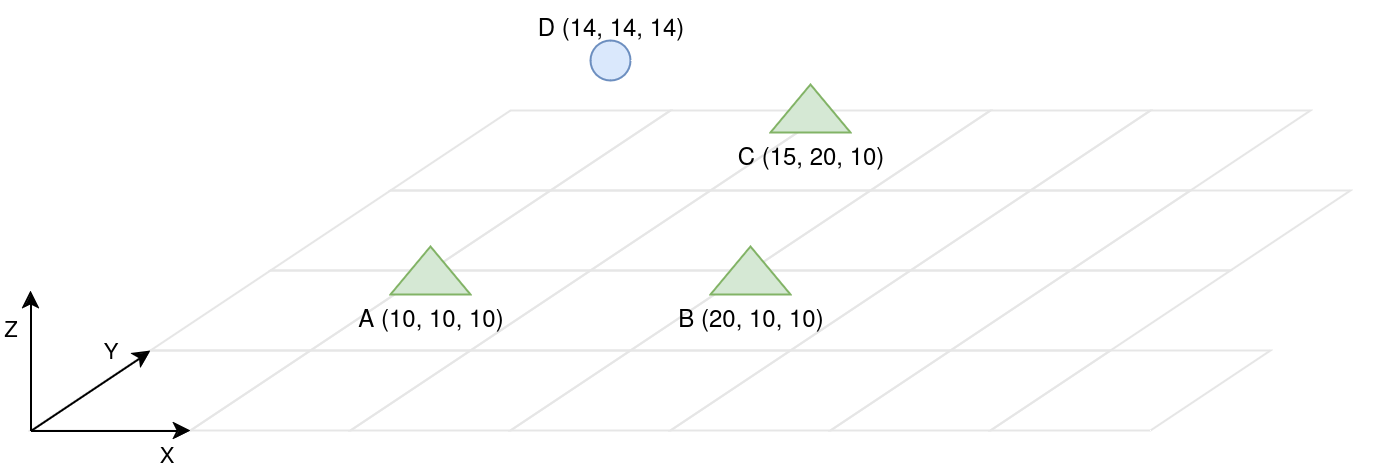
\includegraphics[width=12cm]{Programmer/benchtopo1b.png}
\caption{The 3 fixed points}
\label{fig:topoEx1}
\end{figure}

The summerized content of the GCP file:

\begin{lstlisting}
      <SetGCP>
         <NameSet>"terrain"</NameSet>
         <Measures>
            <el>
               <Name>"A"</Name>
               <Pt>10 10 10</Pt>
               <AdditionalInfo>""</AdditionalInfo>
               <__Opt__Sigma2>.0001 0 0 .0001 0 .0001</__Opt__Sigma2>
            </el>
            <el>
               <Name>"B"</Name>
               <Pt>20 10 10</Pt>
               <AdditionalInfo>""</AdditionalInfo>
               <__Opt__Sigma2>.0001 0 0 .0001 0 .0001</__Opt__Sigma2>
            </el>
            <el>
               <Name>"C"</Name>
               <Pt>15 20 10</Pt>
               <AdditionalInfo>""</AdditionalInfo>
               <__Opt__Sigma2>.0001 0 0 .0001 0 .0001</__Opt__Sigma2>
            </el>
            <el>
               <Name>"D"</Name>
               <Pt>14 14 14</Pt>
               <AdditionalInfo>""</AdditionalInfo>
            </el>
         </Measures>
      </SetGCP>
\end{lstlisting}


\subsection{Creating the observations}

The distances from $D$ to $A$, $B$ and $C$
are measured. For redondancy and error evaluation, the distance from $D$ to $C$ is measured twice
with different values (Fig. \ref{fig:topoEx2}).

\begin{figure}[!h]
\centering
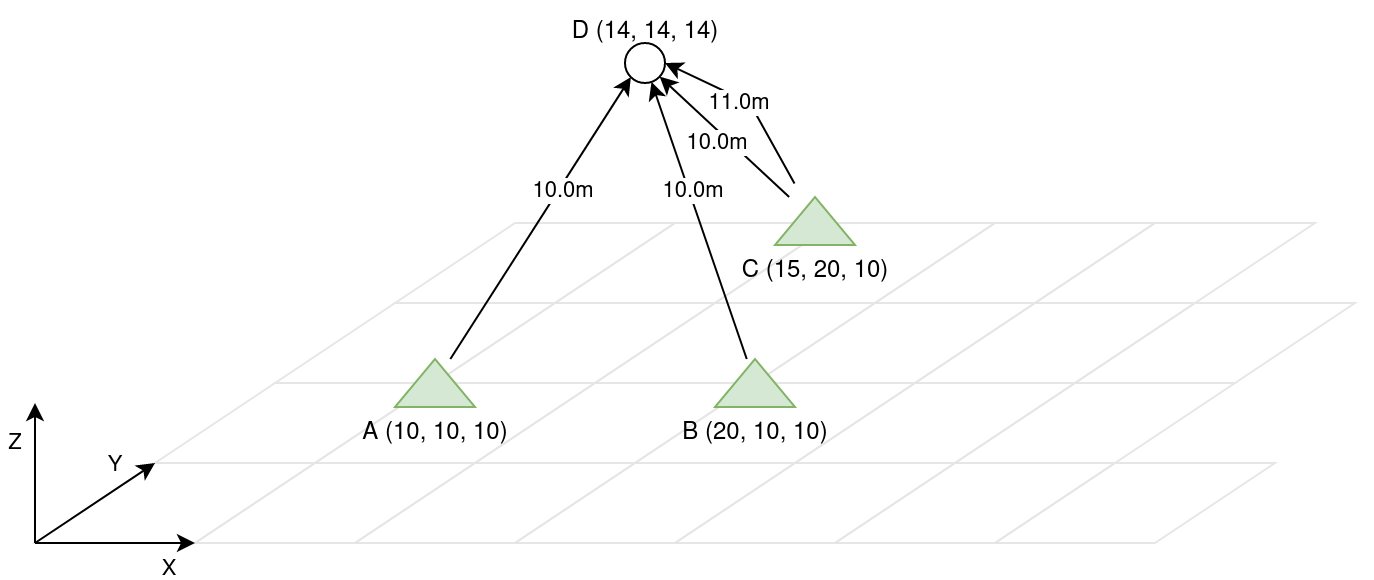
\includegraphics[width=12cm]{Programmer/benchtopo2.png}
\caption{Point $D$ is determined by measured distances}
\label{fig:topoEx2}
\end{figure}

Observations are represented in an {\tt obs} file:
\begin{lstlisting}
    3  D  A  10.0  0.1
    3  D  B  10.0  0.1
    3  D  C  10.0  0.1
    3  D  C  10.1  0.1
\end{lstlisting}

Here a implicit station is created, based on point D.
As no orientation status is given, the station is supposed verticalized.
It should have an horizontal orientation degree of liberty.
But since there is no observations able to determine the station orientation,
it is automatically set as fixed (as if a {\tt \#FIX} line was added at the start of the file).

\subsection{Outputs}

After a computation, the output GCP file contains the final coordinates of every point, including
points that were not declared in the input GCP, but referenced in the survey measurements.

The output Topo file contains info about all the stations and observations,
with output values as residuals:

\begin{lstlisting}
<TopoData>
 <AllObsSetStations>
    <el>
       <TopoObsSetData>
          <Type>"Station"</Type>
          <AllObs>
             <el>
                <TopoObsData>
                   <Type>"Dist"</Type>
                   <Pts>    <el>"D"</el>     <el>"A"</el>       </Pts>
                   <Measures>    <el>10</el>      </Measures>
                   <Sigmas>   <el>0.1</el>     </Sigmas>
                   <__Opt__LastResiduals>  <el>-0.000000000000002</el>  </__Opt__LastResiduals>
                </TopoObsData>
             </el>
[...]
             <el>
                <TopoObsData>
                   <Type>"Dist"</Type>
                   <Pts>      <el>"D"</el>     <el>"C"</el>          </Pts>
                   <Measures>     <el>10.1</el>         </Measures>
                   <Sigmas>       <el>0.1</el>           </Sigmas>
                   <__Opt__LastResiduals>  <el>-0.050000000000001</el>  </__Opt__LastResiduals>
                </TopoObsData>
             </el>
          </AllObs>
          <StationOriStatus>"#FIX"</StationOriStatus>
          <__Opt__Out_G0>0</__Opt__Out_G0>
       </TopoObsSetData>
    </el>
 </AllObsSetStations>
</TopoData>
\end{lstlisting}

This Topo file can be used as input for an other adjustment (it is completely equivalent to the {\tt obs} file).
